\section{Variables to consider when predicting match outcomes}

When predicting the outcome of football matches, there are several variables that can impact the prediction accuracy of a model.

\subsection{Home ground advantage}

Multiple studies have covered the home ground advantage, a phenomenon where several aspects of a match favor the team playing at its home ground.

\citet{bib:courneya-carron-1992} did a state-of-the-art review concerning the home ground advantage, which was reviewed a decade later by \citet{bib:carron-loughead-bray-2005}. \citet{bib:courneya-carron-1992} presented a framework for game location research. \citet{bib:carron-loughead-bray-2005} presented a revised version of the framework, which is shown in \referfigure{fig:carron-loughead-bray-framework}. The framework incorporates five major components, where the factors influence each other from left to right. The components are as follows;
\begin{itemize}
    \item \textbf{Game location}: Simply represents the game site; home versus away. \citet{bib:courneya-carron-1992} suggested that the framework would not work for matches played at neutral grounds, even though one of the teams might be designated as the "home team".
    
    \item \textbf{Game location factors}: Represent four major factors that differently impacts the teams (players and coaches) playing at their own ground versus playing away;
    
    \begin{itemize}
        \item The \textit{crowd factor} is an acknowledgment that the home team has more support from their spectators than the away team has.
        
        Studies have demonstrated how the crowd behavior affects the competing teams, showing that the home team seem to commit more violations when the crowd is showing antisocial behavior (like swearing and throwing objects onto the pitch) \citep{bib:carron-loughead-bray-2005}.
        
        Other studies have shown the effect of the crowd size. The works of \citet{bib:nevill-newell-gale-1996} indicate that absolute crowd size is positively related to the home ground advantage in English and Scottish football. The home teams had an increased home ground advantage in matches where the crowd size was large, while the home ground advantage was nearly absent in two leagues (GM Vauxhall League and Scottish Second Division) where crowd sizes are small \citep{bib:nevill-newell-gale-1996}.
        
        \item The \textit{learning factor} is an acknowledgment that the players playing at home are more familiar with the grounds, and that the club has the ability to temporarily capitalize on their strengths (for example by softening the pitch through extensive watering).
        
        According to \citet{bib:carron-loughead-bray-2005}, studies indicate that teams playing on smaller or larger playing surfaces may have a higher home team advantage than average. Studies also show that teams playing on pitches of artificial grass have a significantly higher home team advantage than average.
        
        The effect of home ground familiarity on the home ground advantage has also been studied. \citet{bib:loughead-carron-bray-kim-2003} collected match information from the English and Scottish Professional Football Associations 1988-2000. They classified matches into three blocks: (a) 10 games immediately before relocating to a new venue; (b) 10 games immediately after relocating to a new venue; and (c) 10 games when the teams had become familiar to the new venue. Before relocating, the teams won $55.2\%$ of their home games. Immediately after relocating, the percentage was reduced to $53.9\%$. After becoming familiar with the new venue, the percentage was virtually unchanged at $53.1\%$ \citep{bib:loughead-carron-bray-kim-2003}. Later on, \citet{bib:loughead-carron-bray-kim-2003} conducted an post-hoc analysis of the results to examine the relationship between team quality and venue familiarity. The findings showed how teams with high home ground advantage suffered significant reductions immediately after moving (i.e. 70.6\% to 59.2\%), while teams with low advantage had the opposite effect (i.e. 34.1\% to 46.8\%).
        
        \item The \textit{travel factor} is an acknowledgment that the away team has to undergo the inconvenience of travelling. 
        
        Studies involving the relationship between home ground advantage and travel distance for the away team have shown that travel distance contribute to the home ground advantage, but that its impact is relatively small \citep{bib:carron-loughead-bray-2005}.
        
        \item The \textit{rule factor} is an acknowledgment that in some sports the rules may favor the home team. This factor does not affect football \citep{bib:carron-loughead-bray-2005}.
    \end{itemize}
    
    \item \textbf{Critical psychological states and Critical behavioural states}: Represent how the psychological and behavioral states of the teams are influenced by game location factors. Focus on the impacts of playing at home ground versus playing away.
    
    According to \citet{bib:carron-loughead-bray-2005}, there are only a few studies concerning the effect of football players' and coaches' psychological states when playing away vs playing at home. One study showed that for male university rugby players, playing at home reduced the level of anxiety, tension, depression, anger, fatigue, etc. The effect of behavioural state has also received little attention \citep{bib:carron-loughead-bray-2005}.
    
    In the initial framework, match officials were also part of the psychological and behavioural states. But seeing as officials do not have home or visitor status, \citet{bib:carron-loughead-bray-2005} removed match officials from the revised framework, and instead looked at them separately.
    
    \item \textbf{Performance outcomes}: Represent how the performance of the teams is influenced by game location, game location factors and the psychological and behavioral states of the teams.
\end{itemize}

\begin{figure}
    \centering
    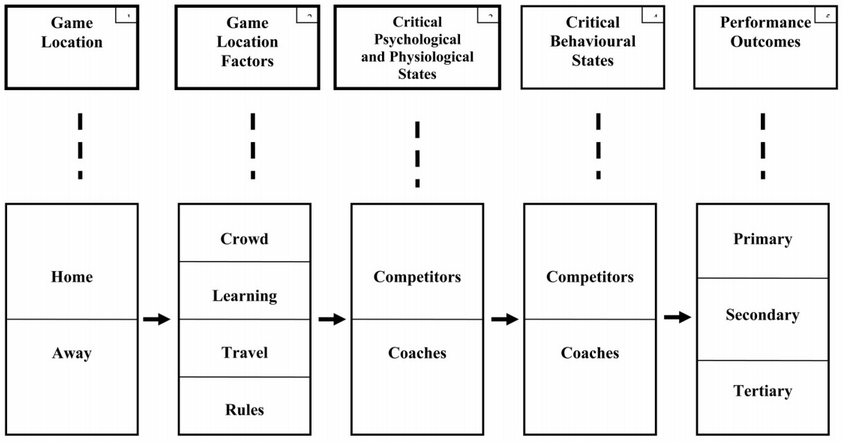
\includegraphics[width=\textwidth]{carron-loughead-bray-framework.png}
    \caption{Framework for game location research. Taken from \citet{bib:carron-loughead-bray-2005}.}
    \label{fig:carron-loughead-bray-framework}
\end{figure}

The framework has been proven useful for providing guidelines on what factors to examine when researching the home ground advantage.

To quantify the home ground advantage, \citet{bib:goddard-2006} collected match results for 35 consecutive seasons in English league football. He looked at the different outcomes of the matches, and how victories are affected by playing at home versus playing away. He also recorded the number of goals scored by the teams over the same period. A summary of his findings is shown in \refertable{tab:goddard-home-results}. The findings clearly show that, even though it has declined the later years, there is still a significant difference between the average performance of the home team and the away team. \citet{bib:bialkowski-lucey-carr-yue-sridharan-matthews-2014} studied teams' style of play. They found that the home team tend to play more in the attacking third of the pitch, which may help explain the difference in number of goals scored between the home and away teams.

There are several other factors influencing the home ground advantage. \citet{bib:pollard-2008} also did a state-of-the-art review on the home ground advantage. He mention how increased travelling distance might increase the home ground advantage, but that the research has shown inconclusive results. The advantage is, however, reduced in local derbies, such as when Arsenal play against Tottenham, two teams with home grounds only $6.6$ km. apart. \citet{bib:pollard-2008} also mention a referee bias. There is evidence that the referee decisions favor the home team. One example is the number of bookings, where the home team is given less bookings that the away team. The bias has been demonstrated in a laboratory setting, where the committed fouls are considered and compared \citep{bib:pollard-2008}. The findings are supported by \citet{bib:nevill-ballmer-williams-2002}, who analyzed 40 referees assessments of an English Premier League match between Liverpool and Leicester City. The referees were exposed to either an audible crowd noise group or no sound at all. The officials in the audible noise group called significantly fewer fouls against the home team than the referees in the silent group. Lastly, \citet{bib:pollard-2008} present research supporting the factors presented in the framework of \citet{bib:carron-loughead-bray-2005}, as well as the special tactics discovered by \citet{bib:bialkowski-lucey-carr-yue-sridharan-matthews-2014}

\begin{table}
    \centering
    \begin{tabulary}{\textwidth}{| L | L | L | L | L |}
        \hline
                                        & \multicolumn{4}{c |}{\textbf{Period}}                                                         \\\hline
        \textbf{Match results (\%)}     & \textbf{1970–1980}    & \textbf{1980–1990}    & \textbf{1990–2000}    & \textbf{2000–2005}    \\\hline\hline
        Home win                        & $50.3$                & $48.8$                & $46.4$                & $45.4$                \\\hline
        Draw                            & $28.6$                & $26.7$                & $27.6$                & $27.5$                \\\hline
        Away win                        & $21.0$                & $24.5$                & $25.9$                & $27.2$                \\\hline\hline
        \textbf{Goals per match (avg.)} &                       &                       &                       &                       \\\hline
        Home team                       & $1.58$                & $1.60$                & $1.51$                & $1.50$                \\\hline
        Away team                       & $0.97$                & $1.06$                & $1.08$                & $1.10$                \\\hline
    \end{tabulary}
    \caption {Trends in home ground advantage in the period 1970-2005. Taken from \citet{bib:goddard-2006}.}
    \label{tab:goddard-home-results} 
\end{table}

\subsection{Attacking and defensive strengths}

Several studies mention the importance of modelling a team's playing abilities, usually in the form of attacking and defensive strengths. However, the way team strengths are modelled have changed over the years.

In the early studies, like that of \citet{bib:maher-1982}, only the number of goals scored and conceded were used for calculating the team strengths. Usually, a team's attacking strength represents their ability to score goals, when their defensive strength represents their ability to avoid conceding goals. \citet{bib:maher-1982} modelled four different strengths for each team; attacking strength when playing at home, defensive strength when playing at home, attacking strength when playing away, and defensive strength when playing away. The distinction between home and away strengths is found in almost every reviewed model, either in the form of separate strengths, or by adding some sort of home ground advantage parameter to the model itself. While the strengths in the model of \citet{bib:maher-1982} do not change over the course of a season, later goal-based studies, like \citet{bib:dixon-coles-1997} and \citet{bib:rue-salvesen-2000}, agree that the strengths of a team vary over time, and that the recent results are more important than older results when modelling the current strengths. Some later models, like that of \citet{bib:cattelan-varin-firth-2013}, focus match outcomes, rather than the number of goals scored. They model a team's strengths at time-step $i$ by the strength at time-step $i-1$ and the number of points achieved in the most recent match.

When adjusting the teams' strengths, the models above do not differentiate "expected" results from those that do not fit the models. For example how lower ranked teams are "expected" to lose against higher ranked teams. The results of a match where the \ordinalnum{1} ranked team loses $0-2$ at home against the \ordinalnum{17} ranked team are treated equally to the results where the \ordinalnum{17} ranked team loses $0-2$ at home against the \ordinalnum{1} ranked team. The probabilities of the two outcomes are quite different, but this difference is not used when adjusting the strengths of the two teams. In the model of \citet{bib:hvattum-arntzen-2010}, the current rank of the two competing teams are taken into account. The difference in rank forms the basis for the ELO rating system.

The system of \citet{bib:constantinou-fenton-neil-2012} takes it a step further. In their system, \citet{bib:constantinou-fenton-neil-2012} do not care about what teams are playing. They consider the teams' current strengths only. To model a team's current strength, \citet{bib:constantinou-fenton-neil-2012} make use of the total number of points accumulated the last three seasons and the number of points accumulated so far the current season, supplemented by the expected number of points for the remaining matches. Team strength is further adjusted using subjective information not captured by previous results (see \refersection{subsec:pi-football}). Another quite unique feature in the model of \citet{bib:constantinou-fenton-neil-2012} is the use of a team's current form. Other models also make use of the recent results of a team, but the model of \citet{bib:constantinou-fenton-neil-2012} measure the recent results of a team according to the expected results, indicating whether a team currently has a good run. In addition, the form is adjusted using the availability of important players.

\subsection{Team characteristics}

Several models try to incorporate the characteristics of football teams in some way. This is usually incorporated in the form of attacking and defensive strengths, number of goals scored per match etc. One shortcoming in these models is the failure to capture how the teams actually play. How do the teams build their attacks? What tactical decisions are made by the teams? These, and similar question, are important to ask, as they are definitive of how the teams play, and thus how the match is played (\citet{bib:pollard-reep-1997}, \citet{bib:bialkowski-lucey-carr-yue-sridharan-matthews-2014}, \citet{bib:hirotsu-wright-2003}).

\subsubsection{Style of play}

\citet{bib:pollard-reep-1997} created a model to capture a team's characteristics. They used a so-called "team possession" as the basic unit of their model. A team possession starts when a player gains possession of the ball, except for when the ball is received from a team member. The receiving player must have good enough control over the ball to be able to deliberately influence the direction of the ball. A team possession ends when one of the following events occur: (a) the ball goes out of play; (b) the ball touches a player of the opposing team (a momentary touch not significantly altering the ball direction is excluded); and (c) an infringement of the rules takes place.

A team possession consists of several components, like passes, throw-ins etc. To assess the effectiveness of the components, the outcome of a team possession need to be quantified. Several outcomes were considered, such as whether the possession ended in a goal, a shot etc. The authors finally composed a outcome measure called "yield". Each outcome is classified by two variables: type of possession and zone of origin. The type of a possession is either free play or set play (like free kicks). The pitch is divided into six different zones, slicing the pitch in equal parts \citep{bib:pollard-reep-1997}.
\begin{equation}
    p_{ij} = \sum_{k=1}^{n_{ij}} \frac{p_{ijk}}{n_{ij}}
    \label{eq:team-possession-probability}
\end{equation}

$p_{ij}$ denotes the probability of scoring after a team possession of type $j$ (1 for open play, 2 for set play) originating in zone $i = 1, ..., 6$. The probability is calculated using \referequation{eq:team-possession-probability}, where $p_{ijk}$ is the $k^{th}$ team possession of type j originating in zone i and $n_{ij}$ is the total number of team possessions of type j originating in zone i. Each recorded team possession is assigned a value $p_{ij}$, defined by the outcome of the possession and the zone of origin of the next team possession. For example, if a team possession ends with the other team regaining the ball in zone 3, then the first team possession will be assigned a value of $-p_{31}$, indicating that the initial team possession ended in favor of the opposing team \citep{bib:pollard-reep-1997}. Using the values $p_{ij}$, the average outcome value for team possessions can be calculated. The average outcome value of a team possession of type j originating in zone i is called the yield $y_{ij}$. The process of setting the values for all $y_{ij}$ is done iteratively.

The yield value can be used to quantify the actual outcome of a team possession. It can also be used to assess the effectiveness of a particular game strategy, by for example taking the mean yield of all team possessions in which the strategy was used. Different strategies can then be compared. \citet{bib:pollard-reep-1997} supplies an example of such a comparison, based on statistics from the World Cup of 1986 in Mexico. The example situation is a throw-in in zone 6. Per 1000 team possessions recorded in the cup, throwing the ball towards the goalmouth had a yield of $21.7$, compared to $3.50$ for a short throw to a nearby team member \citep{bib:pollard-reep-1997}.

\citet{bib:pollard-reep-1997} conclude in their article that fans, media, coaches and players are all sceptical about the suggestion that a statistician might have something useful to provide for a team's tactical analysis, and that a coach's subjective opinions on how to run the game triumphs any number the statistician provide. They suggest using the recorded yields as guidelines on what to base a team's strategy upon. They show examples of actions that provide different yields, such as a zone five free kick; direct shot vs pass to team member, and open field play; running with the ball vs long passes forward vs short passes.

\subsubsection{Team formation}

\citet{bib:bialkowski-lucey-carr-yue-sridharan-matthews-2014} take a closer look on what defines a team's formation, and how it can be identified. Their research question is as following; "Given all the player and ball tracking data of a team in a season, what team-based features can adequately discriminate a team’s behavior?". They answer this question using an in-depth model of a football match, focusing on team formations.

During a match, each player is assigned a role. A given role can only be assigned to one player at any given time, but players may change roles during the match. A role is described by its position relative to the other roles (the left back plays to the left of the central defenders, etc.). A formation assigns a space on the pitch to each player at every time-frame (capturing 10 frames per second). Identifying a team's formation based on player tracking data can be framed as a minimum entropy data partitioning problem \citep{bib:bialkowski-lucey-carr-yue-sridharan-matthews-2014} for each time-frame. An example of such a problem is shown in \referfigure{fig:lee-choi-clustering}. This problem can be modelled as a linear assignment problem, which the authors solve by using the Hungarian algorithm \citep{bib:kuhn-1955}.

\begin{figure}
    \centering
    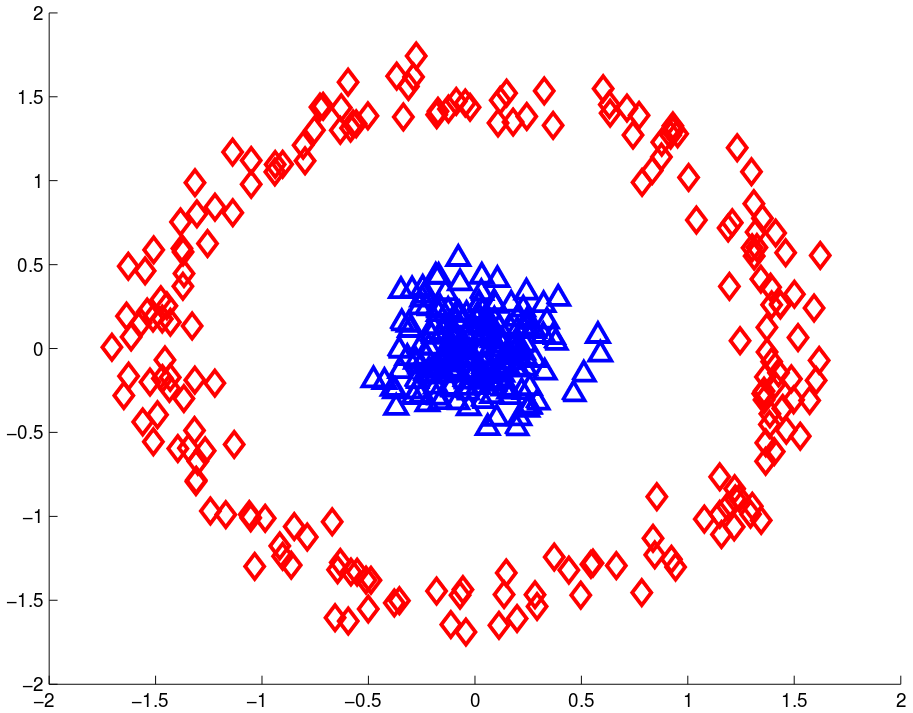
\includegraphics[width=0.75\textwidth]{lee-choi-clustering.png}
    \caption{An example of clustering a ring. Taken from \citet{bib:lee-choi-2004}.}
    \label{fig:lee-choi-clustering}
\end{figure}

Using only player tracking data and ball events for a given team, \citet{bib:bialkowski-lucey-carr-yue-sridharan-matthews-2014} created a model for identifying different teams. The model is based on three different match descriptors;

\begin{itemize}
    \item \textbf{Match statistics:} Various statistics registered during a match. The statistics capture team and individual behavior, and include variables like corners, catches, goals, bookings, chances, shots, etc. Each match statistics event is associated with a timestamp and a location on the pitch.
    \item \textbf{Ball occupancy:} The pitch is divided into a $10x8$ cell big spatial grid. The ball occupancy is calculated for each cell in the grid, and gives a quantitative description of how often the team was in possession of the ball at each cell during a match. This descriptor captures where the different teams like to put pressure during a match. An example of a ball occupancy map is given in \referfigure{fig:bialkowski-et-al-ball-occupancy}. The map shows how the team tend to attack on the left side of the pitch \citep{bib:bialkowski-lucey-carr-yue-sridharan-matthews-2014}.
    \item \textbf{Formation descriptor:} The formation of a team is described as above. The formation description is defined as a $MxN$ matrix, where $M$ is the number of cells in the field and $N$ the number of roles (set to 10, excluding keeper). The descriptor describes where the players of different roles tend to move on the pitch. Ten examples of team formation descriptor depictions are shown in \referfigure{fig:bialkowski-et-al-formation-descriptors}.
\end{itemize}

\begin{figure}
    \centering
    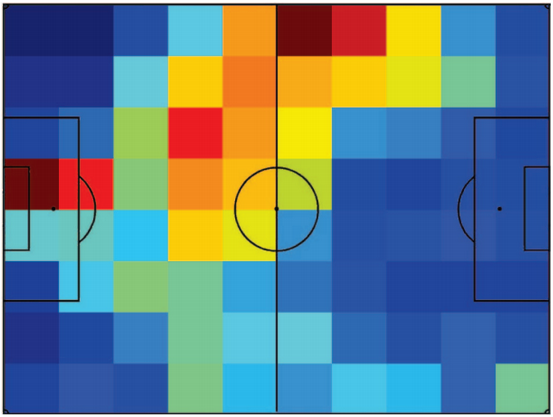
\includegraphics[width=0.75\textwidth]{bialkowski-et-al-ball-occupancy.png}
    \caption{An example ball occupancy map (over a match half) for a team attacking from left to right. Taken from \citet{bib:bialkowski-lucey-carr-yue-sridharan-matthews-2014}.}
    \label{fig:bialkowski-et-al-ball-occupancy}
\end{figure}

\begin{figure}
    \centering
    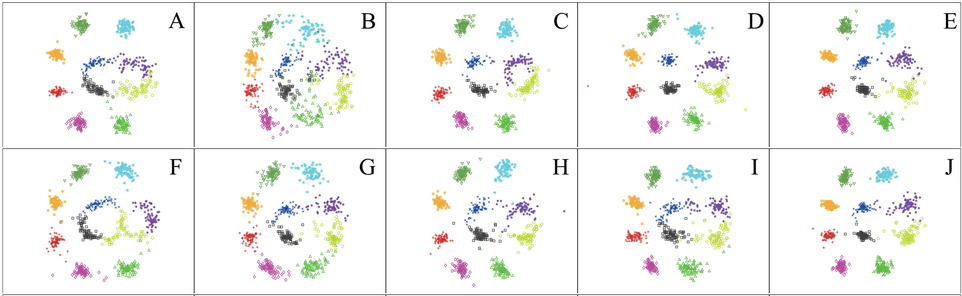
\includegraphics[width=\textwidth]{bialkowski-et-al-formation-descriptors.png}
    \caption{Depictions of team formation descriptors for a team attacking from left to right. The colors represent the different roles. Only the centroid for each role for each match is depicted. Taken from \citet{bib:bialkowski-lucey-carr-yue-sridharan-matthews-2014}.}
    \label{fig:bialkowski-et-al-formation-descriptors}
\end{figure}

\citet{bib:bialkowski-lucey-carr-yue-sridharan-matthews-2014} set up an experiment to test the accuracy of their model. The experiment was conducted using "leave-one-out" cross-validation, training their model on all but one match for each team. Using data from a top-tier professional soccer league, the model correctly predicted the team in over 70\% of the cases. These results clearly show that "teams have a true underlying signal which can be encapsulated in the way the team moves in formation over time" \citep{bib:bialkowski-lucey-carr-yue-sridharan-matthews-2014}. In addition, there is also additional information to gain from where different teams put pressure during matches, and how much they interact with the ball throughout a match. This information, combined with the attacking and defensive strengths of a team, might be useful in prediction of match outcomes \citep{bib:bialkowski-lucey-carr-yue-matthews-2014}. For example, knowing that a team plays a lot on their wings, crossing the ball into the goalmouth, whilst the opposing team has good, strong central defenders might tell something about how the match will progress.

The experiments of \citet{bib:bialkowski-lucey-carr-yue-sridharan-matthews-2014} also showed that teams are rather rigid in the way the play across a season, which they suggest could be used as a powerful prior for preparing for upcoming matches.

Team style is a very subjective and high-level attribute, especially in football, and is therefore hard to segment into discrete parts. Team style covers all aspect of play \citep{bib:bialkowski-lucey-carr-yue-sridharan-matthews-2014}. The way they quantified team style was by computing a linear combination of prior behavior styles. Given a set of team behavior descriptors, they discovered a discrete set of play styles using k-means clustering. Using different values for $k$, completely different patterns were discovered. Every team's style was classified uniquely, with each style modelled as a weighted combination of different styles. This makes sense, as a team might play a pressing game one match, and defending the next \citep{bib:bialkowski-lucey-carr-yue-sridharan-matthews-2014}. \referfigure{fig:bialkowski-et-al-team-style-clusters} shows an example of how different values for $k$ affect the style clustering descriptors. According to \citet{bib:bialkowski-lucey-carr-yue-sridharan-matthews-2014}, these descriptors can be used for predicting the results of future matches.

\begin{figure}
    \centering
    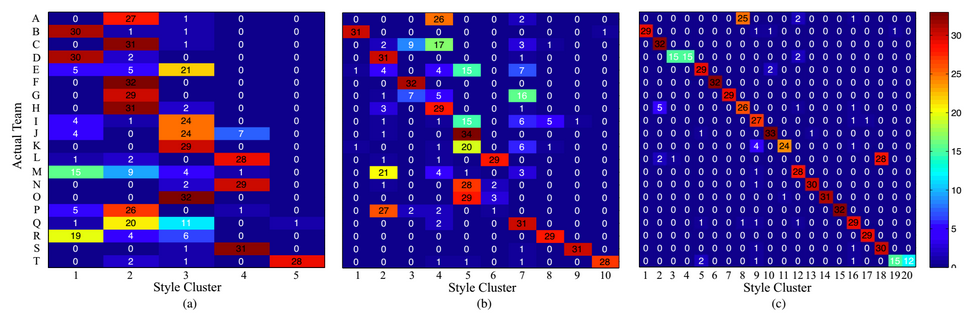
\includegraphics[width=\textwidth]{bialkowski-et-al-team-style-clusters.png}
    \caption{Clustering descriptor of each match half for different values for $k$. (a) 5, (b) 10, (b) 20. Taken from \citet{bib:bialkowski-lucey-carr-yue-sridharan-matthews-2014}.}
    \label{fig:bialkowski-et-al-team-style-clusters}
\end{figure}

In addition to identifying teams based on match data, \citet{bib:bialkowski-lucey-carr-yue-sridharan-matthews-2014} also used the system for predicting team behavior and how matches are played. Given the identities of two opposing teams, they were able to precisely predict the locations of the players in the different roles in most matches. To do this, they used k-NN regression using the learnt team style priors as input. Their predictions estimated with an average of 2 meters error per role for most matches.

In the future, \citet{bib:bialkowski-lucey-carr-yue-sridharan-matthews-2014} plan to use their system for both short-term (who will pass to to etc.) and long-term (match outcome) predictions.


\subsection{Team psychology}

In some cases, the psychology of the competing teams can have an impact on the final results.

\citet{bib:goddard-asimakopoulos-2004} mention the importance of "significant" matches. A match is significant for a team if it is possible (before the match is played) for the team to either win the championship, or to be promoted or relegated, assuming all other teams in contention for the same outcome score one point each on average. According to \citet{bib:goddard-asimakopoulos-2004}, teams are more likely to over-perform in significant matches. As a result, if a match is significant for one team, but not for the other, the incentive difference is likely to influence the final result.

Early elimination from knockout tournaments may also influence a team's results in subsequent league matches. On the one side, a team recently eliminated from a tournament may able to concentrate more on the league, consequently improving their league results. On the other side, elimination might reduce the overall team spirit and confidence of a team, deteriorating the league results. Statistics suggest the latter effect dominates the former \citep{bib:goddard-asimakopoulos-2004}.

\citet{bib:rue-salvesen-2000} mention the effect of superiority. If team A is superior to team B, in terms of team strength and historical results, A tend to underestimate B, changing the outcome probabilities in favor of B. The effect is reversed if A is far too superior, so that B develop an inferiority complex facing A \citep{bib:rue-salvesen-2000}.